\documentclass{beamer}

\usecolortheme[dark,accent=cyan]{solarized}

\beamertemplatenavigationsymbolsempty

\usepackage{graphicx}
\usepackage{hyperref}
\usepackage{colortbl, xcolor}
\usepackage{booktabs}
\usepackage{blindtext} % package for minipage
\usepackage{minted}

\usepackage{tikz}
\usetikzlibrary{calc}

\title{Nikoleta Glynatsi}
\author{@NikoletaGlyn}
\date{2016-02-11}
%\institute[]
%{
%\begin{center}
%    
\includegraphics[width=.15\textwidth]{static/cardiff_uni_logo.jpg}
%\end{center}
%}

\begin{document}

\frame{\titlepage}

\begin{frame}
	\begin{center}
		\huge{Who am I?}
	\end{center}
\end{frame}

\begin{frame}{Who am I?}
\begin{columns}[T] % align columns
\begin{column}{.58\textwidth}
  		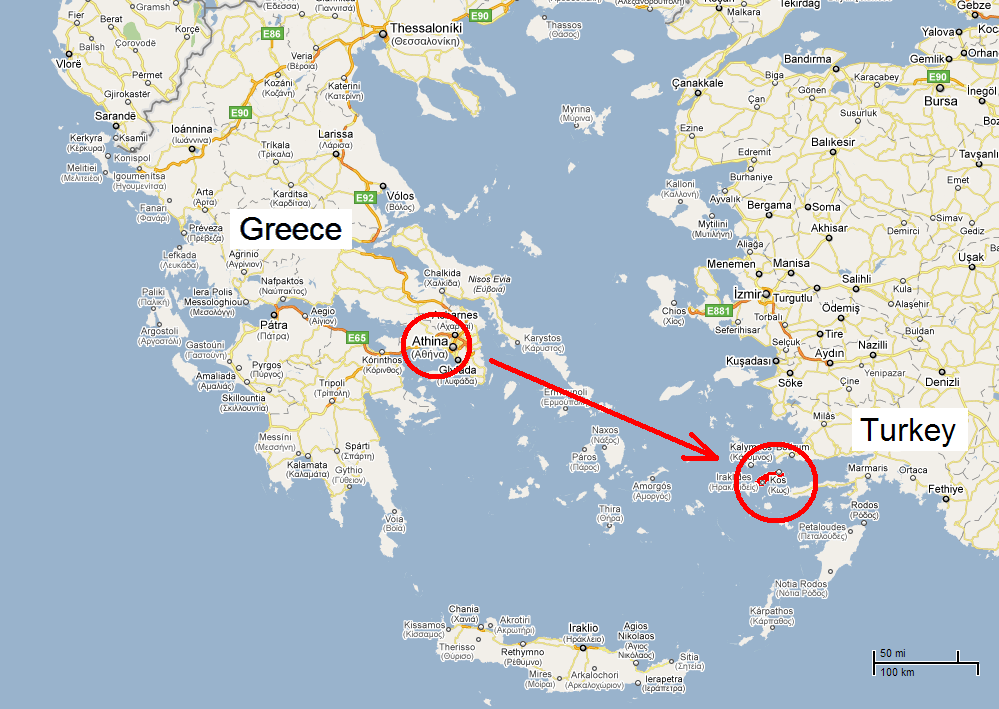
\includegraphics[width=0.8\textwidth]{static/kos-island-map.png}
\end{column}% 
\begin{column}{.38\textwidth}
  		
\includegraphics[width=.30\textwidth]{static/tei-patras-logo.jpg}

  		
\includegraphics[width=.30\textwidth]{static/cardiff_uni_logo.jpg}
\end{column}%
\begin{column}{.38\textwidth}
  		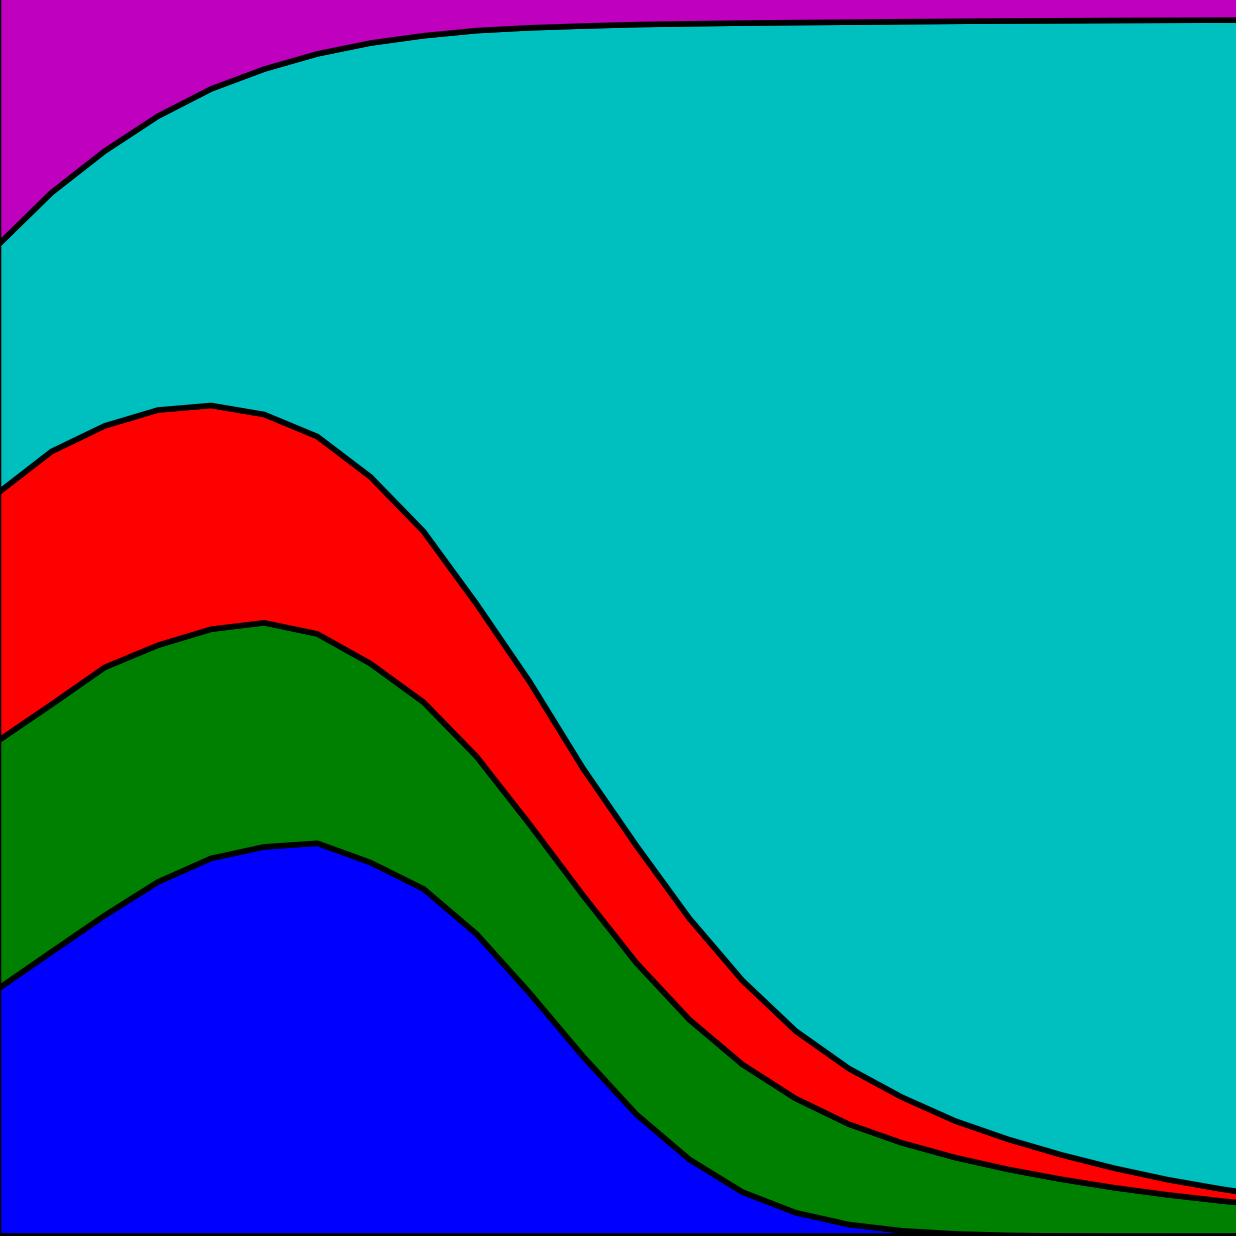
\includegraphics[width=.30\textwidth]{static/axelrod-logo.png}

  		
\includegraphics[width=.30\textwidth]{static/hots_logo.jpg}
\end{column}%
\end{columns}
\end{frame}

\begin{frame}
	\begin{center}
		\huge{What do I do?}
	\end{center}
\end{frame}

\begin{frame}{What do I do?}
\begin{columns}
    \begin{column}{0.30\textwidth}
        \begin{block}{Research}
    {
        \begin{itemize}
        \item Game Theory
        \item Axelrod
        \item Machine Learning
        \end{itemize}
    }
    \end{block}
    \end{column}
    \begin{column}{0.30\textwidth}
        \begin{block}{Groups}
    {
        \begin{itemize}
        \item PyDiff
        \item S.W.O.R.D.S.
        \item PyCon UK
        \item OR Club?!
        \end{itemize}
    }
    \end{block}
    \end{column}
    \begin{column}{0.30\textwidth}
        \begin{block}{Tutoring}
    {
        \begin{itemize}
        \item Computing
        \item Operational Research
        \item Statistics
        \end{itemize}
    }
    \end{block}
    \end{column}   
\end{columns}    
\end{frame}

\begin{frame}{My Plans}
	\begin{center}
		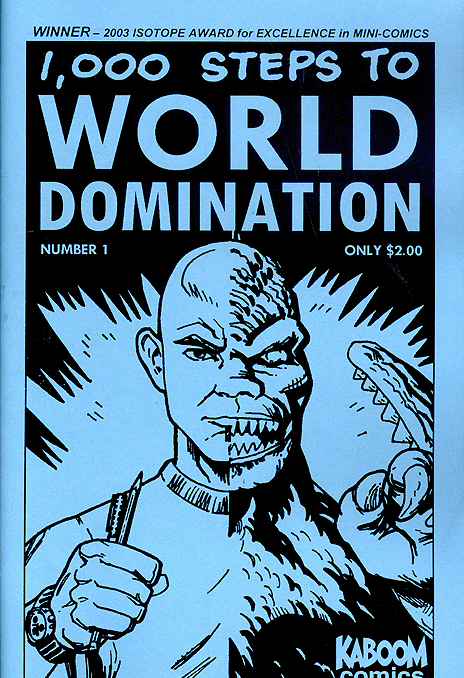
\includegraphics[width=.40\textwidth]{static/evil-mastermind.png}
	\end{center}

\hfill \tiny http://www.sequentialtart.com/reports.php?ID=1971\&issue=2016-08-15

\end{frame}

\begin{frame}
	\begin{center}
		
\includegraphics[width=.80\textwidth]{static/ashlock.png}
	\end{center}
\end{frame}

\begin{frame}
    \begin{block}{Plans:}
    {
        \begin{itemize}
        \item Encourage SSI in my research community
        \end{itemize}
    }
    \end{block}
\end{frame}

\begin{frame}[fragile]{Strategy}
    \begin{center}
        \begin{minipage}{0.8\textwidth}
            \begin{minted}
[
frame=lines,
framesep=2mm,
baselinestretch=1.2,
fontsize=\tiny
]
{python}

>>> import axelrod as axl
>>> me = axl.Human(name='me')
>>> players = [axl.TitForTat(), me]
>>> match = axl.Match(players, turns=3)
>>> match.play() 

Starting new match
Turn 1 action [C or D] for me: C

Turn 1: me played C, opponent played C
Turn 2 action [C or D] for me: D

Turn 2: me played D, opponent played C
Turn 3 action [C or D] for me: C
[('C', 'C'), ('C', 'D'), ('D', 'C')]
            \end{minted}
        \end{minipage}
    \end{center}
\end{frame}

\begin{frame}
    \begin{block}{Plans:}
    {
        \begin{itemize}
        \item Encourage SSI in my research community
        \item Workshops on Game Theory
        \item PyCon UK (including Django girls workshop)
        \item Encourage students 
        \item PyCon Namibia
        \end{itemize}
    }
    \end{block}
\end{frame}

\begin{frame}
	\begin{center}
		\huge{\textbf{}}\\~\\
		\small{@NikoletaGlyn}\\
		\small{https://github.com/Nikoleta-v3}\\
		\small{https://github.com/Axelrod-Python/Axelrod}
	\end{center}
\end{frame}

\end{document}